\documentclass[12pt]{article}
\usepackage{fancyhdr}
\usepackage{amsmath,amsthm,amssymb,dsfont,enumerate,color}
\usepackage[top=1in, bottom=1in]{geometry}
\usepackage{tikz}
\usepackage{tikz-3dplot}
\usetikzlibrary{patterns}
\tdplotsetmaincoords{70}{110}
\usetikzlibrary{arrows.meta}
\fancyhead[L]{MAT473}
\fancyhead[R]{Homework 3}
\fancyfoot[L]{Name: \underline{\hspace{2in}}}
\fancyfoot[R]{\large \thepage}
\fancyfoot[C]{}
\newcommand{\bbA}{\mathbb{A}}
\newcommand{\bbB}{\mathbb{B}}
\newcommand{\bbC}{\mathbb{C}}
\newcommand{\bbD}{\mathbb{D}}
\newcommand{\bbE}{\mathbb{E}}
\newcommand{\bbF}{\mathbb{F}}
\newcommand{\bbG}{\mathbb{G}}
\newcommand{\bbH}{\mathbb{H}}
\newcommand{\bbI}{\mathbb{I}}
\newcommand{\bbJ}{\mathbb{J}}
\newcommand{\bbK}{\mathbb{K}}
\newcommand{\bbL}{\mathbb{L}}
\newcommand{\bbM}{\mathbb{M}}
\newcommand{\bbN}{\mathbb{N}}
\newcommand{\bbO}{\mathbb{O}}
\newcommand{\bbP}{\mathbb{P}}
\newcommand{\bbQ}{\mathbb{Q}}
\newcommand{\bbR}{\mathbb{R}}
\newcommand{\R}{\mathbb{R}}
\newcommand{\bbS}{\mathbb{S}}
\newcommand{\bbT}{\mathbb{T}}
\newcommand{\bbU}{\mathbb{U}}
\newcommand{\bbV}{\mathbb{V}}
\newcommand{\bbW}{\mathbb{W}}
\newcommand{\bbX}{\mathbb{X}}
\newcommand{\bbY}{\mathbb{Y}}
\newcommand{\bbZ}{\mathbb{Z}}
\newcommand{\bbk}{\mathbb{k}}

\newcommand{\calA}{\mathcal{A}}
\newcommand{\calB}{\mathcal{B}}
\newcommand{\calC}{\mathcal{C}}
\newcommand{\calD}{\mathcal{D}}
\newcommand{\calE}{\mathcal{E}}
\newcommand{\calF}{\mathcal{F}}
\newcommand{\calG}{\mathcal{G}}
\newcommand{\calH}{\mathcal{H}}
\newcommand{\calI}{\mathcal{I}}
\newcommand{\calJ}{\mathcal{J}}
\newcommand{\calK}{\mathcal{K}}
\newcommand{\calL}{\mathcal{L}}
\newcommand{\calM}{\mathcal{M}}
\newcommand{\calN}{\mathcal{N}}
\newcommand{\calO}{\mathcal{O}}
\newcommand{\calP}{\mathcal{P}}
\newcommand{\calQ}{\mathcal{Q}}
\newcommand{\calR}{\mathcal{R}}
\newcommand{\calS}{\mathcal{S}}
\newcommand{\calT}{\mathcal{T}}
\newcommand{\calU}{\mathcal{U}}
\newcommand{\calV}{\mathcal{V}}
\newcommand{\calW}{\mathcal{W}}
\newcommand{\calX}{\mathcal{X}}
\newcommand{\calY}{\mathcal{Y}}
\newcommand{\calZ}{\mathcal{Z}}
\newcommand{\iitem}{\vfill \item}
\newcommand{\topic}[1]{\textcolor{blue}{#1}}
\newcommand{\answerbox}{\begin{flushright}
    \begin{tikzpicture}
      \draw (0,0) rectangle (5,-1.75);
    \end{tikzpicture}\end{flushright}}
\newcommand{\solution}[1]{\textcolor{red}{#1}}
\newcommand{\points}[1]{\ [#1pts]}
%\renewcommand{\solution}[1]{}

\begin{document}
\pagestyle{fancy}

Throughout we assume that $R$ is a commutative ring with identity
$1\neq 0$.
\begin{enumerate}
\item Recall that $S^{-1}R$ is defined to be the set of equivalence
  classes in $R\times S$ with the equivalence relation $(r,s)\sim
  (r',s')$ if there exists an element $t\in S$ such that
  $t(rs'-r's)=0$. Prove that the multiplication $(r_1,s_1)\cdot
  (r_2,s_2)=(r_1r_2,s_1s_2)$ is a well-defined operation on
  $S^{-1}R$. 
\item Define $\Phi$ to be the
  function which takes a subset of $R$ to a subset of $S^{-1}R$ in the
  following way: 
  \[\Phi(I) = \{(x,s) \mid x\in I, s\in S\}.\]
  \begin{itemize}
  \item Prove that if $I$ is an ideal in $R$, then $\Phi(I)$ is an
    ideal in $S^{-1}R$. 
  \item Prove that if $P$ is a prime ideal that does not intersect
    $S$, and $S$ has no zero divisors, then $\Phi(I)$ is a prime ideal
    in $S^{-1}R$. 
  \end{itemize}


\item Suppose that $S\subset R$ is a multiplicative set in $R$. Prove
  that the homomorphism $\phi: R\rightarrow S^{-1}R$ is injective if
  and only if $S$ contains no zero-divisors. 
\item Let $p$ be a prime integer, and consider the ring $R=\bbZ$. Let
  $S=\bbZ \setminus p\bbZ$. The ring $S^{-1}R$ is called the
  localization of $\bbZ$ at $p$. Find all of the ideals of this ring,
  and describe the maximal ideal (there is only one).
\item This problem is to help us look ahead. Let $\varphi(n)$ denote
  the number of units in $\bbZ/n\bbZ$. (From previous homework, we
  know this is the same as computing the number of integers $1\leq k<n$
  that are relatively prime to $n$.)
\begin{enumerate}
\item Compute $\varphi(p^k)$ when $p$ is prime and $k$ is a
  non-negative integer.
\item Compute $\varphi(n)$ for $n\in \{6, 10, 12, 18, 24, 36\}$ and make a
  conjecture about the relationship between $\varphi(n)$ and the prime
  power decomposition of $n$. 
\end{enumerate}

\end{enumerate}
Here I'll recall the universal property that defines a product, and
introduce a new one that defines the coproduct. 

\fbox{\begin{minipage}{0.95\linewidth}
{\bf Definition:} Let $X_1, X_2$ be objects in a category $\calC$. Define $X_1 \prod X_2$
  to be the object with the following universal property: There are
  morphisms $\pi_i: X_1\prod X_2 \rightarrow X_i$ such that if there
  is any other object $T$ with morphisms $\varphi_i: T\rightarrow X_i$
  for $i\in \{1,2\}$, then there is a unique morphism $\Psi:
  T\rightarrow X_1 \times\prod X_2$ such that $\pi_i \circ \Psi =
  \varphi_i$. 
\end{minipage}}

\begin{minipage}{0.55\linewidth}This is conveniently captured in the diagram to the right, and is read to mean that you start with the
  object $X_1 \prod X_2$ and its morphisms to $X_1$ and $X_2$ set in
  stone. Any time there is an object $T$ with morphisms as in the
  diagram, there is a morphism $\Psi$ that can fill in that dotted
  arrow so that the diagram commutes, meaning any two ways to get to
  the same place produce the same morphism. 
\end{minipage} \begin{minipage}{0.4\linewidth}
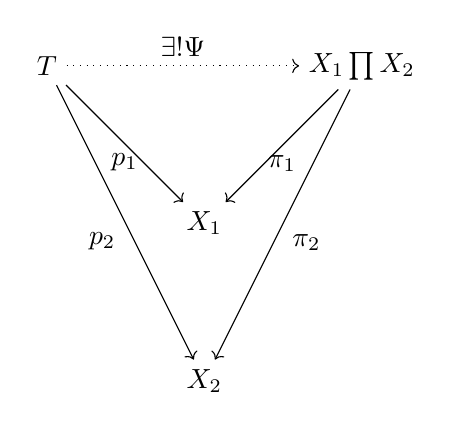
\begin{tikzpicture}
    \node (T) at (-2,0) {$T$};
    \node (prod) at (2,0) {$X_1 \prod X_2$};
    \node (X1) at (0,-2) {$X_1$};
    \node (X2) at (0,-4) {$X_2$};
    \draw[->] (T)--(X1) node[midway, below] {$p_1$};
    \draw[->] (T)--(X2) node[midway, below left] {$p_2$};
    \draw[->] (prod)--(X1) node[midway, below] {$\pi_1$};
    \draw[->] (prod)--(X2) node[midway, below right] {$\pi_2$};
    \draw[dotted,->] (T)--(prod) node[midway, above] {$\exists ! \Psi$};
  \end{tikzpicture}\end{minipage}
\begin{enumerate}
\item[6.] Prove that if $R_1$ and $R_2$ are rings, then the
  product ring $\{(r_1,r_2) \mid r_1\in R_1, r_2\in R_2\}$ is actually
  the object $R_1 \prod R_2$. I.e., verify that it satisfies the
  universal property. 
\item[7.] Consider now the category $\calC$ whose objects are positive
  integers and so that $\operatorname{Mor}_\calC(n,m) =\begin{cases}
    \{m/n\} & \textrm{ if } m\mid n\\
\emptyset & \textrm{ otherwise}\end{cases}.$ Given two integers $n,m$,
compute $m \prod n$ in this context (i.e., what integer has the
desired universal property). 
\end{enumerate}
If you really like the last problem, awesome. You can try your hand at
a new one. This is just for the superfans. Try to write what you think
the universal property of the coproduct should be given just the
diagram: 

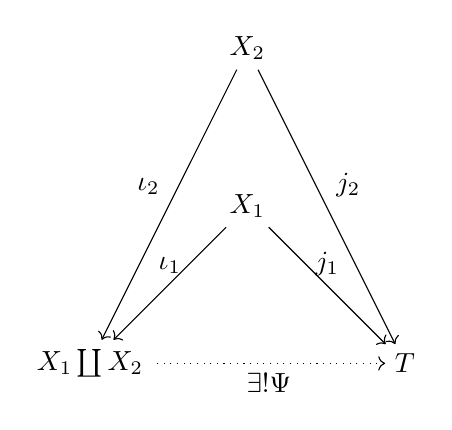
\begin{tikzpicture}
      \node (T) at (2,0) {$T$};
    \node (prod) at (-2,0) {$X_1 \coprod X_2$};
    \node (X1) at (0,2) {$X_1$};
    \node (X2) at (0,4) {$X_2$};
    \draw[<-] (T)--(X1) node[midway, above] {$j_1$};
    \draw[<-] (T)--(X2) node[midway, above right] {$j_2$};
    \draw[<-] (prod)--(X1) node[midway, above] {$\iota_1$};
    \draw[<-] (prod)--(X2) node[midway, above left] {$\iota_2$};
    \draw[dotted,<-] (T)--(prod) node[midway, below] {$\exists ! \Psi$};
\end{tikzpicture}

Then, compute $m\coprod n$ for objects $m,n$ in $\calC$. 
\end{document}
2018/01/17 18:53:34
